\section*{Teoretická část}
\subsection*{Kundtova trubice}
Budeme měřit rychlost zvuku v kovové tyči pomocí Kundtovy trubice.
Kundtova trubice je z jedné strany uzavřená skleněná trubice, z druhé strany do ní vložíme tyč ze zkoumaného materiálu, kterou na konci opatříme korkovým pístem.
Do trubice rovnoměrně rozprostřeme korkový prášek a tyč podélně rozkmitáme.
Pokud v trubici vzniklo stojaté vlnění, prášek vytvoří obrazec naznačený na obrázku \ref{obr::obrazectrubice}.
Pokud stojaté vlnění nevzniklo, změníme vzdálenost mezi koncem trubice a korkovým pístem a opakujeme, dokud nevznikne.
Vzdálenost mezi dvěma nejbližšími místy, kde písek nebyl rozmetán, je rovna polovině vlnové délky zvuku.

\begin{figure}[htbp]
\centering
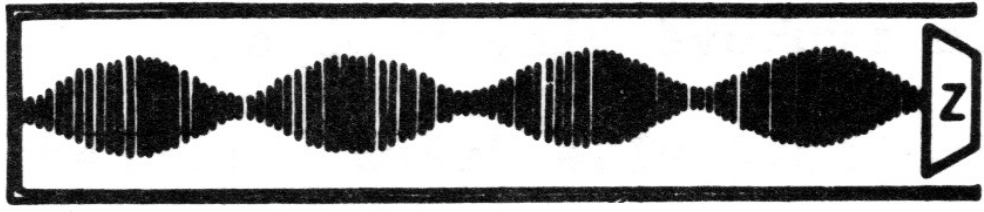
\includegraphics[width=\textwidth-10cm]{graficos/obr1}
\caption{Rozmetaný písek v Kundtově trubici}
\label{obr::obrazectrubice}
\end{figure}

Kovovou tyč o délce $l_T$ upevníme v jejím prostředku, pak bude vydávat zvuk o vlnové délce $\lambda_1$ rovné dvojnásobku svojí délky, platí tedy
\begin{equation} \label{eq::lambda1tyc}
\lambda_1=2 \cdot l_T  \,.
\end{equation}

Při přechodu z jednoho prostředí do druhého si zvuk zachovává svojí frekvenci
\begin{equation} \label{eq::kundt_rovnost_frekvenci}
f_1= \frac{c_1}{\lambda_1}=\frac{c_2}{\lambda_2}=f_2 \,.
\end{equation}
kde $f$ je frekvence, $c$ je rychlost zvuku a dolní indexy 1 a 2 označují prostředí (tyč, vzduch resp.).
Ze známé rychlosti zvuku ve vzduchu a změřených $\lambda_1$, $\lambda_2$ můžeme snadno určit rychlost šíření ve zkoumané tyči.

Pro tenkou tyč platí \cite{ZFP}
\begin{equation}
c_1 = \sqrt{ \frac{E}{\rho}  } \,,
\end{equation}
kde $E$ je modul pružnosti v tahu a $\rho$ je hustota tyče.
Při známé rychlosti zvuku v tyči a její hustoty můžeme vypočítat modul pružnosti v tahu
\begin{equation} \label{eq::modulpruznosti}
E=c_1^2 \cdot \rho \,.
\end{equation}

\subsection*{Uzavřený rezonátor}
Uzavřený rezonátor je uzavřená dutá kovová trubice s nastavitelnou délkou.
Na jednom jejím konci je připevněn reproduktor napojený na elektronický tónový generátor, na druhém konci je mikrofon napojený na mikroampérmetr.
Rezonance nastává vždy, když je délka rezonátoru celočíselný násobek poloviny vlnové délky zvuku:
\begin{equation} \label{eq::l_na_k}
l=k \cdot \frac{\lambda}{2} \,,  \qquad  k=1, 2, 3, \ldots
\end{equation}
po úpravě
\begin{equation} \label{eq::f_na_k}
f=\frac{c}{2l} \cdot k \,.
\end{equation}

Pokud rezonance nastane, zaznamenáme na mikroampérmetru jako lokální maximum.
Rezonátor je opatřen uzavíratelnými přívody, kterými do něj můžeme napustit měřený plyn.

Rychlost zvuku v plynu budeme měřit dvěma způsoby:
\begin{itemize}
\item S konstantní délkou oscilátoru budeme měnit frekvenci zdroje. Naměřenou závislost \eqref{eq::f_na_k} nafitujeme přímkou $f(k) = a \cdot k$. Z konstanty $a$ určíme rychlost zvuku jako
\begin{equation} \label{eq::cza}
c = 2 \cdot a \cdot l
\end{equation}
\item Při konstantní frekvenci zdroje budeme měnit délku rezonátoru. Po úpravě \eqref{eq::f_na_k} máme
\begin{equation} \label{eq::zavislost_l}
l= \frac{c}{2f} \cdot k  \,.
\end{equation}
Tuto naměřenou závislost nafitujeme přímkou $l(k)= b \cdot k$. Porovnáním s \eqref{eq::zavislost_l} dostaneme
\begin{equation} \label{eq::czb}
c = 2 \cdot f \cdot b \,.
\end{equation}
\end{itemize}

Rychlost zvuku ve vzduchu budeme měřit oběma způsoby.
Rychlost v oxidu uhličitém budeme měřit pouze při konstantní délce rezonátoru.

V plynu je rychlost zvuku určena Laplaceovým vzorcem \cite{ZFP}
\begin{equation}
c_2 = \sqrt{\kappa \frac{p}{\rho}} \,,
\end{equation}
kde $\kappa$ je Poissonova konstanta, $p$ je tlak plynu a $\rho$ jeho hustota.
Dosazením ze stavové rovnice a následnou úpravou dostaneme
\begin{equation} \label{eq::kappa}
\kappa = \frac{c^2 \mu}{RT} \,,
\end{equation}
kde $R=~\SI{8.314}{\joule\per\kelvin\per\mole}$ je molární plynová konstanta, $T$ je teplota v kelvinech a $\mu$ je molární hmotnost plynu.

\emph{Poznámka:~}Pro lineární regresi $y = ax$ sady nezávislých proměnných $x_i$ a závislých $y_i$ se standardní odchylkou $\sigma_i$ počítáme koeficient $a$ podle vzorce \cite{prakt}
\begin{equation}
a=\frac{ \sum_{i=1}^{n} \frac{y_ix_i}{\sigma_i^2}
}{\sum_{i=1}^{n} \frac{x_i^2}{\sigma_i^2}  }
 \qquad \qquad \sigma_a^2=\frac{1}{
 \sum_{i=1}^{n} \frac{x_i^2}{\sigma_i^2}}
\end{equation}

